% vim: set spelllang=en :

\documentclass[10pt]{article}

\usepackage{amsmath, amssymb, amsfonts, amsthm} 
\usepackage{upgreek} 
\usepackage{amsthm} 
\usepackage{fullpage}
\usepackage{graphicx}
\usepackage{cancel}
\usepackage{wrapfig}
\usepackage{subfigure}
\usepackage{mathrsfs}
\usepackage{outlines}
\usepackage[font={sf,it}, labelfont={sf,bf}, labelsep=space, belowskip=5pt]{caption}
\usepackage{hyperref}
\usepackage{titling}
\usepackage{xifthen}
\usepackage{color}
\usepackage{fancyhdr}
\usepackage[title]{appendix}
\usepackage{float}
\usepackage{enumitem}

\usepackage{bm}
\usepackage{minted}
\usepackage{xcolor}

\pagestyle{fancy}
\headheight 24pt
\headsep    12pt
\lhead{\documenttitle}
\rhead{\today}
\fancyfoot[C]{}
\lfoot{}
\rfoot{\thepage}
\renewcommand{\headrulewidth}{0.4pt}
\renewcommand\footrulewidth{0.4pt}
\newcommand{\documenttitle}{Assignment Solution}
\newcommand{\coursetitle}{SE2324: Mathematical Foundation of Computer Sciences(Spring 2021)}
\newcommand{\authorname}{Zihong Lin, 519021911327} % Your name and ID here

\makeatletter

\setlength{\droptitle}{-50pt}

\title{\documenttitle \vspace{1ex} \\ \Large \coursetitle \vspace{-1ex}}
\author{\authorname\vspace{-1ex}}


% BEGIN DOCUMENT
\begin{document}
\maketitle


%%%%%%%%%%%%%%%%%%%
\section{README}

... 

%%%%%%%%%%%%%%%%%%%
\section{NumPy Warm-up (15 points)}

Consider the following one-dimensional \textit{Gaussian probability distribution}, also known as the Normal distribution or bell curve distribution:

\begin{center}
$
G(x \mid \mu, \sigma)=\frac{1}{Z} \exp \left[-\frac{1}{2} \frac{1}{\sigma^{2}}(x-\mu)^{2}\right] \quad
$
where 
$
Z=\sqrt{\frac{\pi}{\frac{1}{2} \frac{1}{\sigma^{2}}}}
$
\end{center}

Here, the function $G : \mathbb{R} \rightarrow \mathbb{R}$ takes as input a scalar $x$, and produces as output a scalar. 
The particular bell shape of $G$ is determined by two parameters: the mean $\mu \in \mathbb{R}$ and the variance $\sigma^2 \in \mathbb{R}$

Numerically verify the following identity in Python:

\begin{center}
$\int_{\mathbb{R}} G(x) d x=1$
\end{center}

\begin{enumerate}[label=2.\arabic*]
    \item (10 points)
    Choose a few different one-dimensional Gaussian functions (by choosing different mean and variance values), plot them.\par
    Draw four gaussian distribution graph based on 3$\sigma$-rule, the four graphs are shown as follows:\par
    \begin{figure}[htbp]
    	\centering
    	\begin{minipage}[c]{0.5\textwidth} %minipage????????0.2????0.2
    		\centering
    		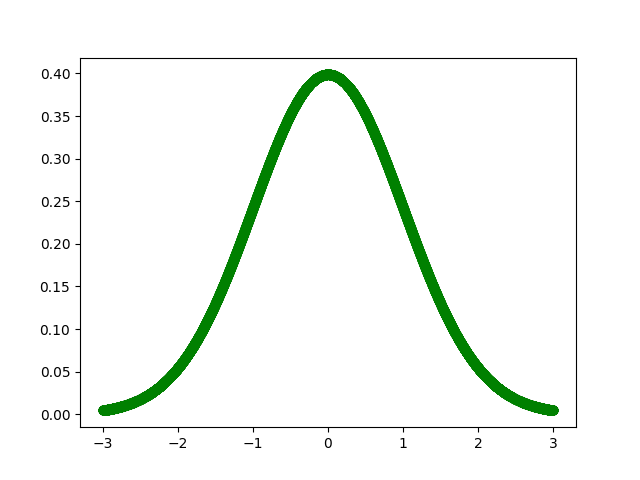
\includegraphics[width=1\linewidth]{./gaussian/0.png}
    		\caption{Gaussian Distribution($\mu=0\ and\ \sigma=1$)}
    	\end{minipage}%
    	\begin{minipage}[c]{0.5\textwidth}
    		\centering
    		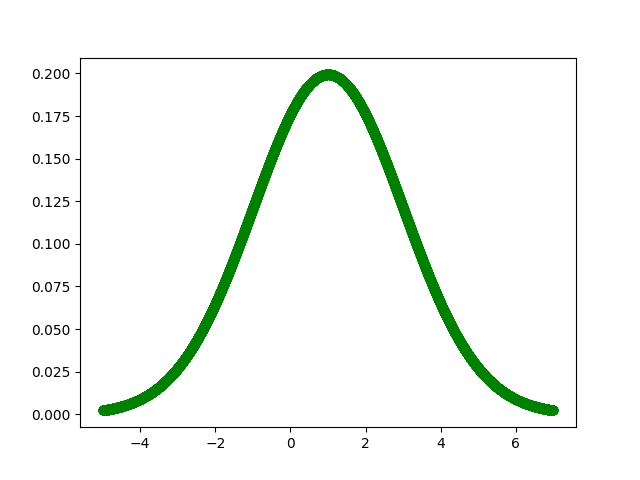
\includegraphics[width=1\textwidth]{./gaussian/1.png}
    		\caption{Gaussian Distribution($\mu=1\ and\ \sigma=2$)}
    	\end{minipage}
    \end{figure}
	\begin{figure}[htbp]
 	\centering
 	\begin{minipage}[c]{0.5\textwidth} %minipage????????0.2????0.2
 		\centering
 		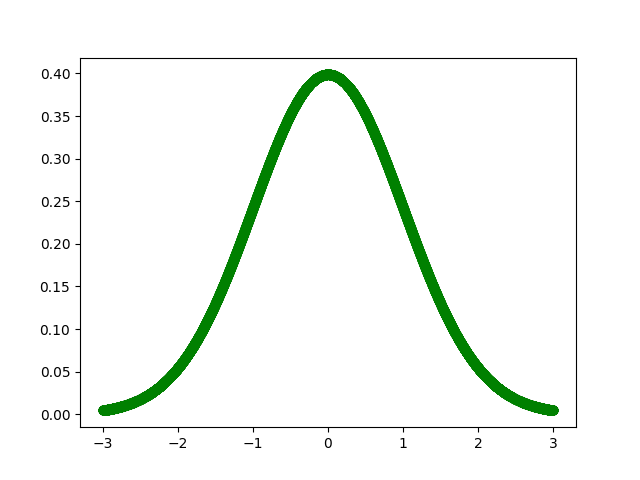
\includegraphics[width=1\linewidth]{./gaussian/0.png}
 		\caption{Gaussian Distribution($\mu=5\ and\ \sigma=0.5$)}
 	\end{minipage}%
 	\begin{minipage}[c]{0.5\textwidth}
 		\centering
 		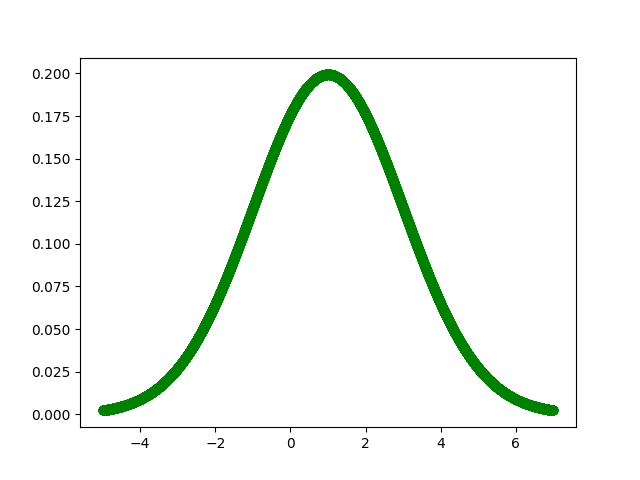
\includegraphics[width=1\textwidth]{./gaussian/1.png}
 		\caption{Gaussian Distribution($\mu=10\ and\ \sigma=4$)}
 	\end{minipage}
 	\end{figure}
 	Put them together:\par
	\begin{figure}[H]
 		\centering
 		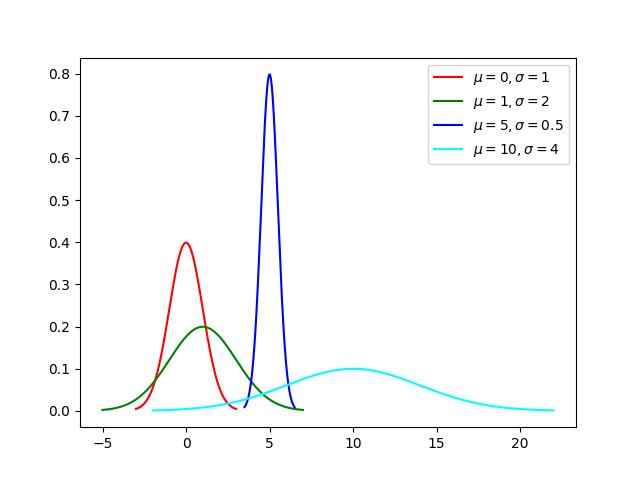
\includegraphics[width=1\textwidth]{./gaussian/together.png}
 		\caption{Gaussian Distribution}
 	\end{figure}
    \item (10 points)
    Verify the above identity for each Gaussian function.\par 
    Using knowledge of calculus,I write a programme to verify the above identity for the four function mentioned above.The running result of the programme are as follows:\par
   	\begin{figure}[H]
    	\centering
    	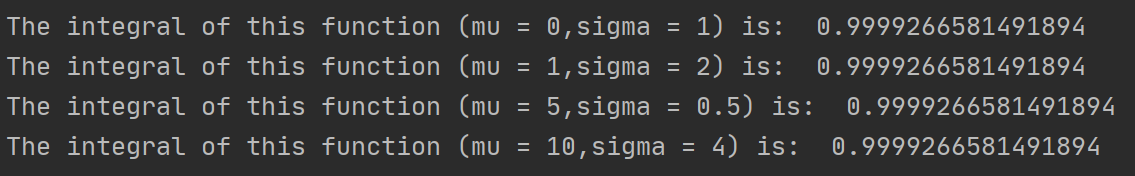
\includegraphics[width=1\textwidth]{./gaussian/result_1.png}
    	\caption{Running result of the programme}
    \end{figure}
	The integral region is $[\mu - 4\sigma,\mu + 4\sigma]$,according to the attributions of gaussian function,the result would be extremely close to 1.Apparently,with the region strenching,the result would infinitely approach to 1,which numerically verify the above identity.\par
	Then I try to use Kahan Algorithm to reduce error,the running results are as follows:\par
	\begin{figure}[H]
		\centering
		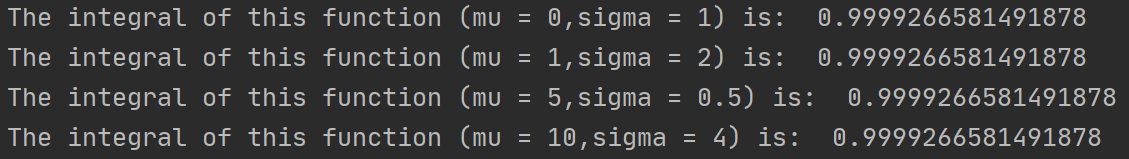
\includegraphics[width=1\textwidth]{./gaussian/result_2.png}
		\caption{Running result of the programme}
	\end{figure}
	The result would be much more precise with the help of kahan algorithm.
\end{enumerate}



%%%%%%%%%%%%%%%%%%%
\section{Numerics and Linear Algebra (60 points)}\label{sec:num_lin_alg}

In this question, you will explore how the condition number of a matrix can have practical influence on which algorithms (e.g. LU, Cholesky) you can use to solve linear systems of the form: $A\vec{x}=\vec{b}$ where $A\in \mathbb{R}^{n\times n}$.
We will study the Vandermonde matrix, as well as a matrix constructed from a finite Fourier Series basis.
In this question, you will interpolate samples of the analytical function

\begin{center}
$f(x)=\frac{1}{1+x^2}$    
\end{center}

for $x\in[0,1]$. Your monomial interpolants (with $N=n+1$ terms) are given by

\begin{center}
$g_V(x)=\sum_{j=0}^{N} c_j x^j$
\end{center}

and

\begin{center}
$g_{F}(x)=\sum_{j=1}^{N / 2} c_{j} \sin (j \pi x)+\sum_{j=N / 2+1}^{N} c_{j} \cos ((j-N / 2) \pi x)$.
\end{center}

Use $M=m+1$ uniformly sampled positions

\begin{center}
$x_i=ih,\text{ }i=0\dots m$,
\end{center}

with spacing $h=1/m$, to generate $M$ samples of the test function $f$,

\begin{center}
$f_i=f(x_i),\text{ }i=0\dots m$.
\end{center}

To estimate the polynomial coefficients $\vec{c}$, you will assemble and solve the linear systems

\begin{center}
$V\vec{c}=\vec{f}$
\end{center}

and

\begin{center}
$F\vec{c}=\vec{f}$
\end{center}

where $V$ is the M-by-N Vandermonde matrix with entries

\begin{center}
$V_{ij}=(x_i)^j$
\end{center}

and $F$ is the finite Fourier Series basis matrix with entries

\begin{center}
$F_{i, j-1}=\left\{
    \begin{array}{ll}
        \sin \left(j \pi x_{i}\right), & \text { if } 1 \leq j \leq N / 2 \\
        \cos \left((j-N / 2) \pi x_{i}\right), & N / 2+1 \leq j \leq N
    \end{array}
\right.$
\end{center}

For simplicity, assume $M=N$ for the entire problem.

\begin{enumerate}[label=3.\arabic*]
    \item (25 points) \label{q:3.1}
    Use an LU solve (\textit{scipy.linalg.lu} from SciPy package) to estimate the monomial coefficients $\vec{c}$. (You can solve a linear system $A
    \vec{x}=\vec{b}$ using NumPy API \textit{numpy.linalg.solve}().)
    Report the residual L2 norm ($||r||_2=||Ax-b||_2$) for both linear systems when $N = 8$ and $N = 16$.\par
    I choose to use the function linalg.lu with parament permute\_l = False,which will calculate the matrices: P,L,U(P refers to permutation). With matrix P, the calculation would avoid deviding zero or a very tiny number.\par
    This function will factorize the vandermonde matrix V into P, L and U, namely $N=PLU$\par
    Thus the linear function $Vc=f$ would become $PLUc=f$ ,namely $LUc=P^{-1}f$\par
    Then one function has been split into two:$Ly=M(let\ M = P^{-1}f)$ and $Uc=y$. Solving out these two function, then we will get the coeffecient matrix $c$\par
    By doing so, the original $O(n^3)$ gaussian elimination algorithm has become $O(n^2)$, which is much more efficient.The residual L2 norm is shown as follows, the algorithm's performance is pretty good.\par 
    	For problem 4.1, the result is:\par
    \begin{table}[H]
    	\centering
    	\begin{tabular}{|l|l|l|}
    		\hline
    		$Matrix$& $N$ & $Residuals$  \\ \hline
    		$V$& $8$ & $7.02\times 10^{-16}$  \\ \hline
    		$F$& $8$ & $6.11\times 10^{-16}$ \\ \hline
    		$V$& $16$ & $2.28\times 10^{-15}$  \\ \hline
    		$F$& $16$ & $1.82\times 10^{-15}$ \\ \hline
    	\end{tabular}
    	\caption{Results of using LU Factorization}
    \end{table}
    When N = 8, for matrix V: 
    \begin{equation}      
    c=\left(                 
    \begin{array}{cccccccc}
    1.0000&-0.0002&-0.9643&-0.2559&1.9341&-1.8375&0.7290&-0.1034
    \end{array}
    \right)^T              
    \end{equation}
    for matrix F:
    \begin{equation}      
    c=\left(                 
    \begin{array}{cccccccc}
    1.3549&-0.0412&-0.3543&0.0016&0.2605&0.8306&-0.0106&-0.0806
    \end{array}
    \right)^T              
    \end{equation}
    When N = 8, for matrix V: 
    \begin{equation}      
    c=\left(                 
    \begin{array}{c}
     1.3556\\2.67\times 10^{-7}\\-1.0000\\2.94\times 10^{-4}\\0.9963\\0.0031\\-1.1759\\0.7328\\-1.2524\\5.1317\\-9.5698\\10.1178\\-6.7019\\2.7954\\-0.0678\\ 0.0074
    \end{array}
    \right)             
    \end{equation}
    for matrix F:
    \begin{equation}      
    c=\left(                 
    \begin{array}{c}
    1.4290\\-0.0056\\-0.0669\\0.0009\\0.0146\\-7.09\times 10^{-4}\\-0.0009\\1.01\times 10^{-5}\\0.0270\\1.0564\\-0.0023\\-0.0350\\0.0003\\0.0045\\-1.19\times 10^{-4}\\ -9.87\times 10^{-4}
    \end{array}
    \right)              
    \end{equation}
    \begin{figure}[H]
    	\centering
    	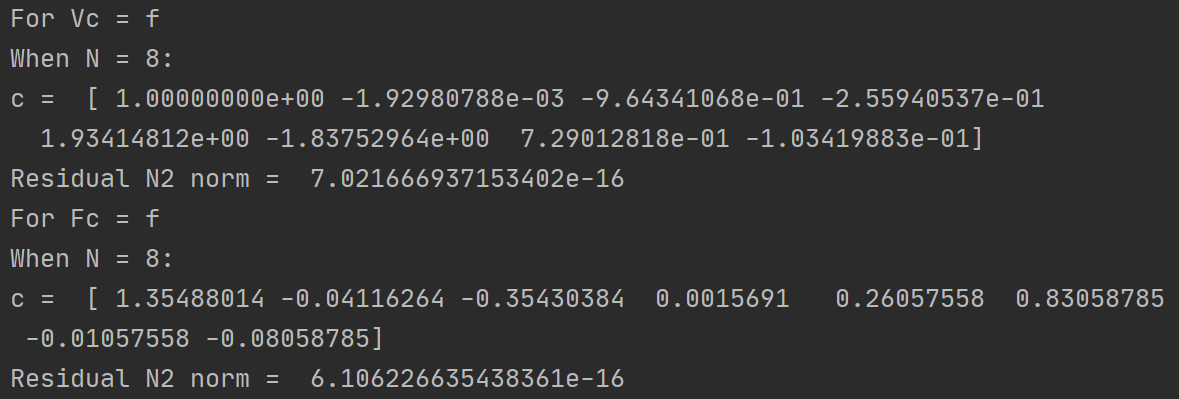
\includegraphics[width=1\textwidth]{./linear algebra/result_1.png}
    	\caption{Running result of the programme}
    \end{figure}
	\begin{figure}[H]
		\centering
		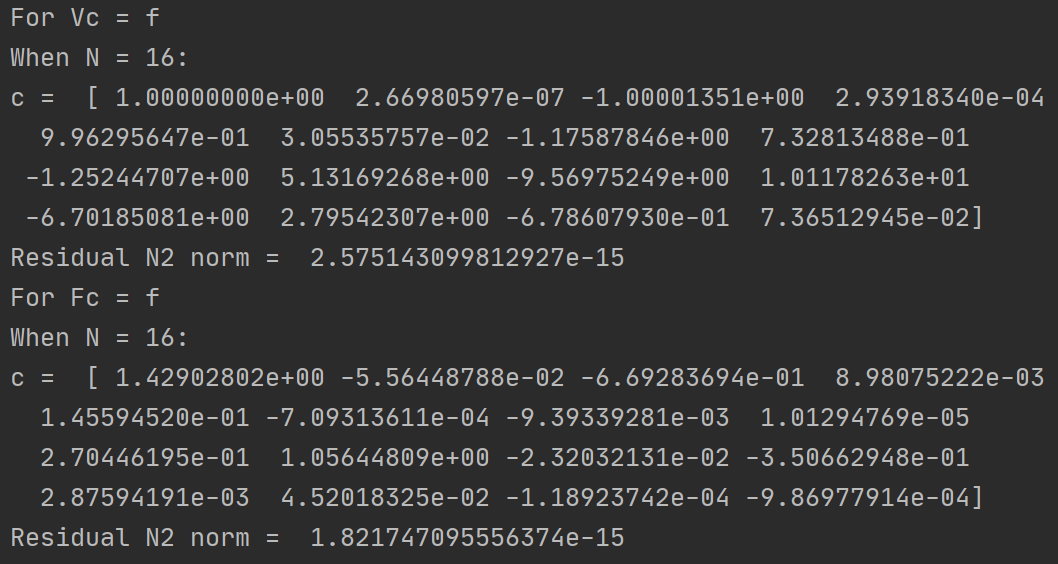
\includegraphics[width=1\textwidth]{./linear algebra/result_2.png}
		\caption{Running result of the programme}
	\end{figure}
    \item (10 points)
    Using the \textit{numpy.linalg.cond} function in NumPy, plot $N$ vs. $cond(V)$ and $N$ vs. $cond(F)$ for $N = 4, 6, 8, ...32$. 
    Write a couple of sentences explaining the reasons for the trends in these two plots. Hints: Use a logarithmic scale in y axis for better clarity. Also, try wrapping the creation of $V$ and $F$ into functions that you can call repeatedly to generate the required output data. These functions will be helpful for the next part.\par
    The graph of cond(V) and cond(F) is shown as follows:\par
    For linear function $Ax = b$, $cond(A)$ can determine how sensitive the function is. A very big condition number means that very tiny changes of b would lead to greate change of x\par 
    Both $cond(V)$ and $cond(F)$ explodes with N increasing, that's because when N become too big, overfitting would usually occur. When overfitting, a tiny change will make big differences, the system is rather sensitive, thus possessing high condition number.\par
    In addition, fourier series fit the function $f(x)=\frac{1}{1+x^2}$ better than polynomial. Thus, facing tiny changes, it's system is less sensitive, which means lower condition number. That explains why $cond(F)$ is always lower than $cond(V)$
   	\begin{figure}[H]
   	\centering
   	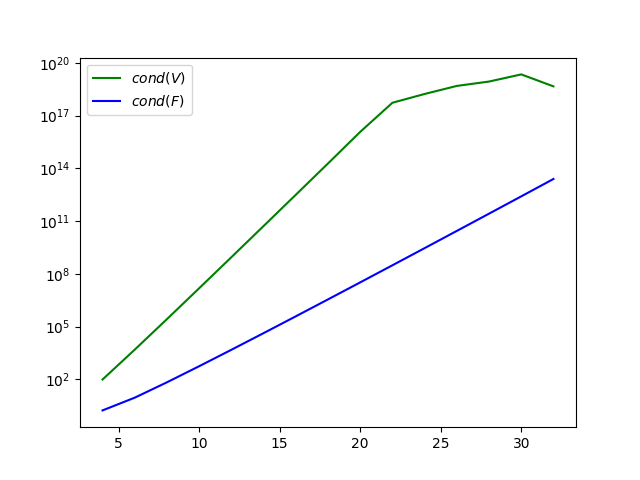
\includegraphics[width=1\textwidth]{./linear algebra/cond.png}
   	\caption{$cond(V)\ and\ cond(F)$}
    \end{figure}
    \item (15 points) \label{q:3.3}
    A necessary condition for being able to use Cholesky factorization is that the matrix must be positive definite. 
    Construct $A_V = V^TV$ and $A_F = F^TF$ for $N = 4, 6, \dots32$ (a total of 30 matrices). 
    Mathematically, when would these matrices be positive definite? Explain.
    Using the \textit{isposdef}() function introduced in Appendix \ref{app:posdef}, check to which matrices NumPy reports as positive definite. Create a table of values that includes the following columns: $N$, \textit{isposdef}($A_V$), \textit{isposdef}($A_F$), cond($V$), cond($F$).
    What is the largest value of $N$ where $A_V$ is positive definite, and what is the condition number of that $V$? 
    What is the largest value of $N$ where $A_F$ is positive definite, and what is the condition number of that $F$? 
    Are these condition numbers connected in some way? If so, how?\par
    	When the colomn vectors of A are linearly dependent, $A^TA$ is positive definite.\par
    Proof: Assume that $A=(a_1,a_2,...,a_k)$, A is reversible.\par
    \begin{equation}       %开始数学环境
    B=\left(                 %左括号
    \begin{array}{cccc}   %该矩阵一共3列,每一列都居中放置
    {a_1}^Ta_1 & {a_1}^Ta_2&... & {a_1}^Ta_n\\  %第一行元素
    {a_2}^Ta_1 & {a_2}^Ta_2&... & {a_2}^Ta_n\\  %第一行元素
    ... & ...&... & ...\\  %第一行元素
    {a_n}^Ta_1 & {a_n}^Ta_2&... & {a_n}^Ta_n\\  %第一行元素
    \end{array}
    \right)=A^TA                 %右括号
    \end{equation}
    A is reversible, so $\forall x\neq0,Ax=0$ has no root.\par
    $x^TBx=x^TA^TAx=(Ax)^T(Ax)=||Ax||^2>0$,so B is positive definite, otherwise, it's semi-definite.\par
    The table is shown as follows:\par
    \begin{table}[H]
    	\centering
    	\begin{tabular}{|l|l|l|l|l|}
    		\hline
    		$N$& $isposdef(A_V)$ &$isposdef(A_F)$  &$cond(V)$  &$cond(F)$  \\ \hline
    4  & True  & True  & 98.86773850722766      & 1.7320508075688772 \\ \hline
    6  & True  & True  & 4924.37105661106       & 9.171872237725903  \\ \hline
    8  & True  & True  & 267816.70090760005     & 68.55137085190168  \\ \hline
    10 & True  & True  & 15193229.677049411     & 562.7580822445406  \\ \hline
    12 & True  & True  & 883478686.1836076      & 4830.611029146824  \\ \hline
    14 & False & True  & 52214922517.12616      & 42680.75493211507  \\ \hline
    16 & False & True  & 3121662403201.779      & 385010.13412784704 \\ \hline
    18 & False & True  & 188254229022756.3      & 3528111.5213114736 \\ \hline
    20 & False & True  & 1.1722528631537054e+16 & 32732760.078300484 \\ \hline
    22 & False & True  & 5.307811978221406e+17  & 306733651.4763673  \\ \hline
    24 & False & False & 1.6732639550599708e+18 & 2898148517.412925  \\ \hline
    26 & False & False & 4.809361466442202e+18  & 27573128629.336758 \\ \hline
    28 & False & False & 8.513196516565954e+18  & 263875678112.03745 \\ \hline
    30 & False & False & 2.1702851332170723e+19 & 2537780703596.8345 \\ \hline
    32 & False & False & 4.5302818866969103e+18 & 24653374108576.676 \\ \hline
    	\end{tabular}
    \end{table}
	The largest value of N where $A_V$ is positive definite is 12, the condition number of that V is 883478690.28;	The largest value of N where $A_F$ is positive definite is 22, the condition number of that V is 306733651.48; These codition numbers are connected in some way, for they are in the same order of magnitude.
    \item (10 points)
    For $N = 8$, transform the linear systems above into positive definite systems according to Question \ref{q:3.3}, and use Cholesky factorization (\textit{numpy.linalg.cholesky}()) to solve them. Report the residual L2 norm for each solution. Compare the residuals to Question \ref{q:3.1}: how does Cholesky compare to LU?
	The results of calculation are as follows:
	\begin{table}[H]
		\centering
		\begin{tabular}{|l|l|l|l|}
			\hline
			$Matrix$& $N$ &$method$ & $Residuals$  \\ \hline
			$V$& $8$ &$LU\ Factorization$& $7.02\times 10^{-16}$  \\ \hline
			$V$& $8$ &$Cholesky\ Factorization$& $5.47\times 10^{-11}$ \\ \hline
			$F$& $8$ &$LU Factorization$& $6.11\times 10^{-16}$  \\ \hline
			$F$& $8$ &$Cholesky\ Factorization$& $1.48\times 10^{-15}$ \\ \hline
		\end{tabular}
		\caption{Results of using Cholesky Factorization}
	\end{table}
	When N = 8 and using Cholesky Factorization, for matrix V: 
	\begin{equation}      
	c=\left(                 
	\begin{array}{cccccccc}
	1.0000&-0.0002&-0.9643&-0.2559&1.9341&-1.8375&0.7290&-0.1034
	\end{array}
	\right)^T              
	\end{equation}
	for matrix F:
	\begin{equation}      
	c=\left(                 
	\begin{array}{cccccccc}
	1.3549&-0.0412&-0.3543&0.0016&0.2605&0.8306&-0.0106&-0.0806
	\end{array}
	\right)^T              
	\end{equation}
	\begin{figure}[H]
		\centering
		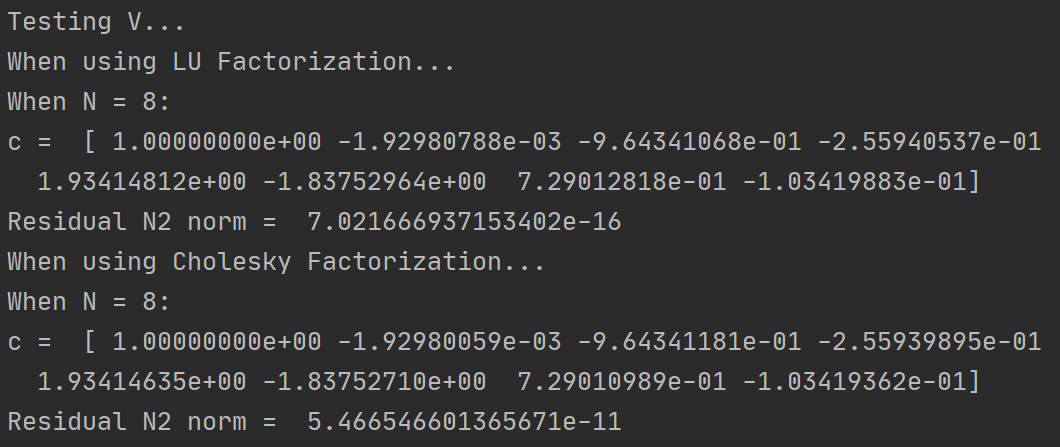
\includegraphics[width=1\textwidth]{./linear algebra/result_3.png}
		\caption{Running result of the programme(For V)}
	\end{figure}
	\begin{figure}[H]
		\centering
		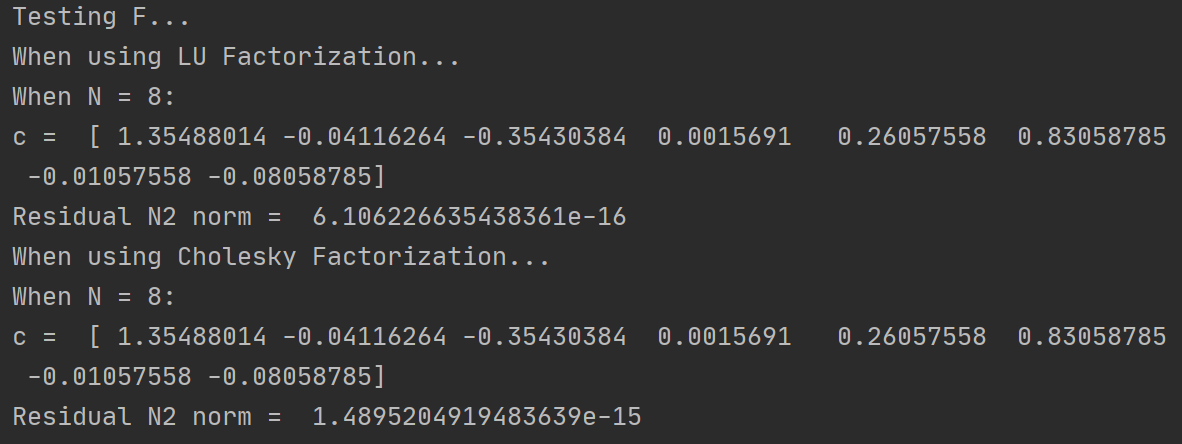
\includegraphics[width=1\textwidth]{./linear algebra/result_4.png}
		\caption{Running result of the programme(For F)}
	\end{figure}
	In this problem, LU Factorization causes lower residuals than Cholesky Factorization. But Cholesky store less infomation than LU, the former need to store a matrix L, while the latter need to store L and U.\par
\end{enumerate}
	

%%%%%%%%%%%%%%%%%%%
\section{Least Squares Problems and QR (25 points)}\label{sec:lin_lsp}

In the question above, a $M\times M$ square linear system is solved for the interpolation coeffcients.
The resulting interpolation function can provide a solution that pass through all the sample points.
However, in some applications, finding such a solution could be too time-consuming and unnecessary, or even impossible (Consider two sample with the same $x$ value and different $y$ values).
In such cases, we usually reduce the number of the interpolants (let $M>N$), and solve the resulting over-determined linear system using least square method.
Instead of looking for the exact solution to an over-determined system, we look for the solution with the smallest error vector $V\vec{c}-\vec{f}$ (or $F\vec{c}-\vec{f}$) by minimizing the overall backward error:

\begin{center}
minimize $\|V \vec{c}-\vec{f}\|_{2}^{2}$
\end{center}

\begin{enumerate}[label=4.\arabic*]
    \item (15 points)
    Solve the least square system with QR decomposition(\textit{numpy.linalg.qr}()) when $M=16$, $N=4,8$.\par
	For problem 4.1, the result is:\par
	\begin{table}[H]
		\centering
		\begin{tabular}{|l|l|l|}
			\hline
			$Matrix$& $N$ & $Residuals$  \\ \hline
			$V$& $4$ & $0.0058$  \\ \hline
			$F$& $4$ & $0.40$ \\ \hline
			$V$& $8$ & $1.77\times10^{-5}$  \\ \hline
			$F$& $8$ & $0.016$ \\ \hline
		\end{tabular}
		\caption{Results of using QR Factorization}
	\end{table}
	When N = 4, for matrix V: 
	\begin{equation}      
	c=\left(                 
	\begin{array}{cccc}
	1.0017&-0.0270&-1.0191&0.5470   
	\end{array}
	\right)^T              
	\end{equation}
	for matrix F:
	\begin{equation}      
	c=\left(                 
	\begin{array}{cccc}
	1.2367&-0.0248&0.2476&0.5393  
	\end{array}
	\right)^T              
	\end{equation}
	When N = 8, for matrix V: 
	\begin{equation}      
	c=\left(                 
	\begin{array}{ccccccccc}
	1.0000&-0.0001&-0.9758&-0.2001&1.8013&-1.6719&0.6252&-0.0776
	\end{array}
	\right)^T              
	\end{equation}
	for matrix F:
	\begin{equation}      
	c=\left(                 
	\begin{array}{cccccccc}
	1.3556&-0.0426&-0.3631&0.0020&0.2617&0.8350&-0.0117&-0.0881 
	\end{array}
	\right)^T              
	\end{equation}
	\begin{figure}[H]
		\centering
		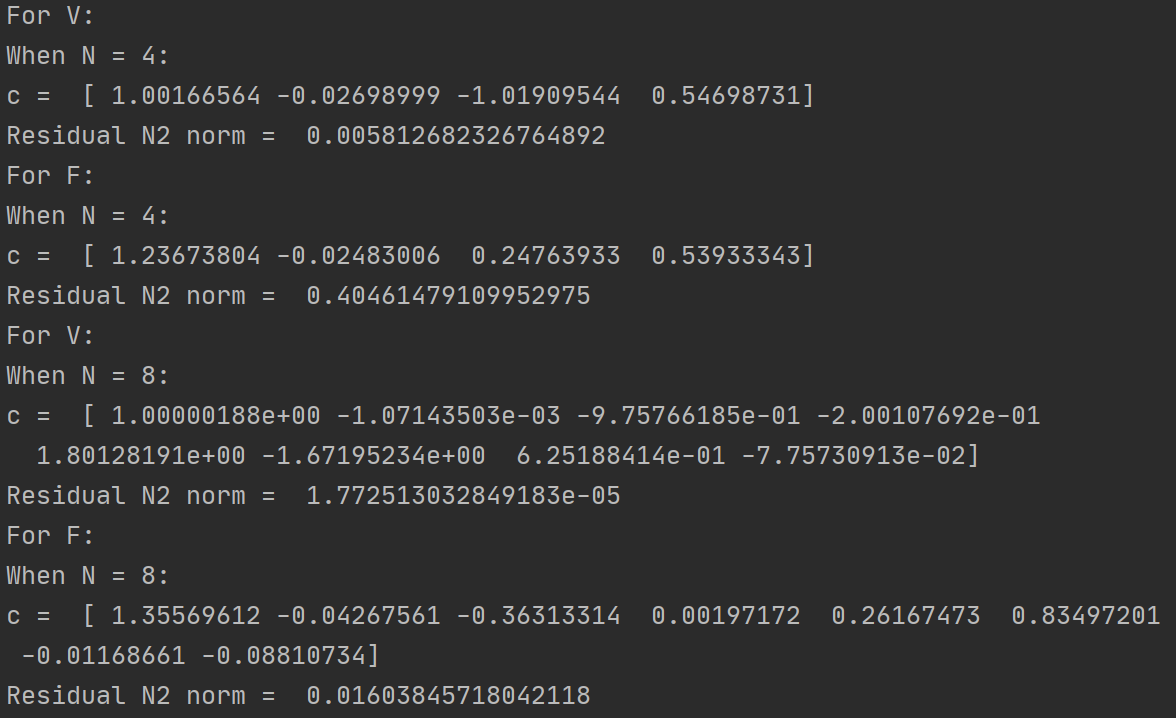
\includegraphics[width=1\textwidth]{./linear algebra/result_5.png}
		\caption{Running result of the programme}
	\end{figure}
    \item (10 points)
    Plot the $g_V$, $g_F$ when $M=16$, $N=4,8$, compare them with the analytical function $f(x)$ and the interpolation function obtained in Question \ref{q:3.1}.\par
    	The graphs are as follows:(predict refers to the given function)\par
    \begin{figure}[H]
    	\centering
    	\begin{minipage}[c]{0.45\textwidth} 
    		\centering
    		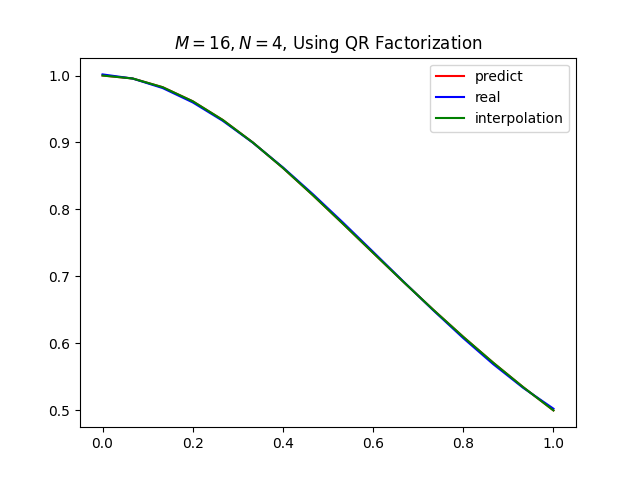
\includegraphics[width=1\textwidth]{./QR/M=16N=4V.png}
    		\caption{$g_V(M=16,N=4)$}
    	\end{minipage}%
    	\begin{minipage}[c]{0.45\textwidth}
    		\centering
    		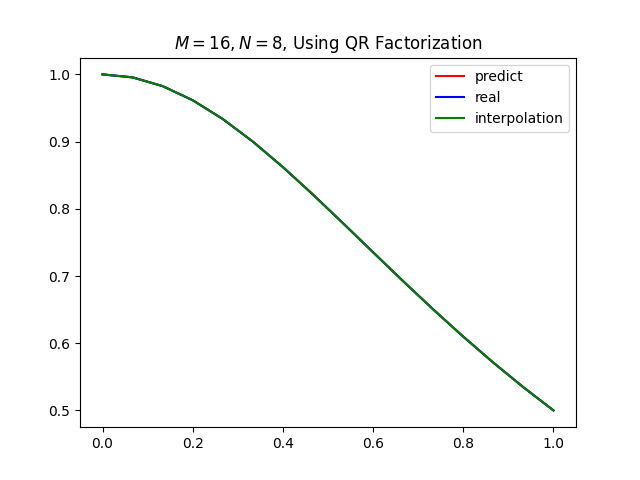
\includegraphics[width=1\textwidth]{./QR/M=16N=8V.png}
    		\caption{$g_V(M=16,N=8)$}
    	\end{minipage}
    \end{figure}
    \begin{figure}[H]
    	\centering
    	\begin{minipage}[c]{0.45\textwidth}
    		\centering
    		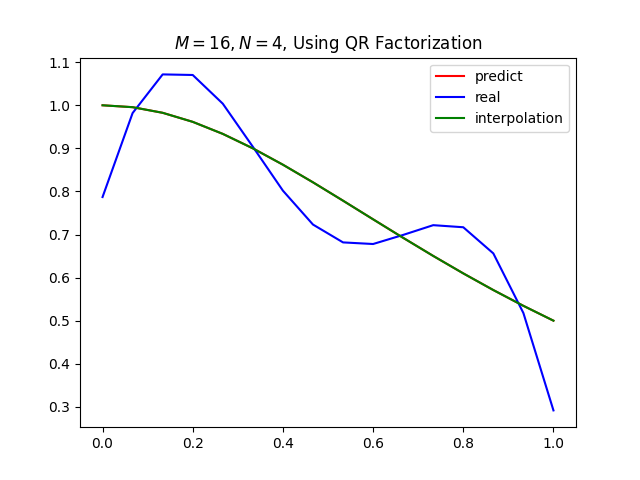
\includegraphics[width=1\textwidth]{./QR/M=16N=4F.png}
    		\caption{$g_F(M=16,N=4)$}
    	\end{minipage}
    	\begin{minipage}[c]{0.45\textwidth} 
    		\centering
    		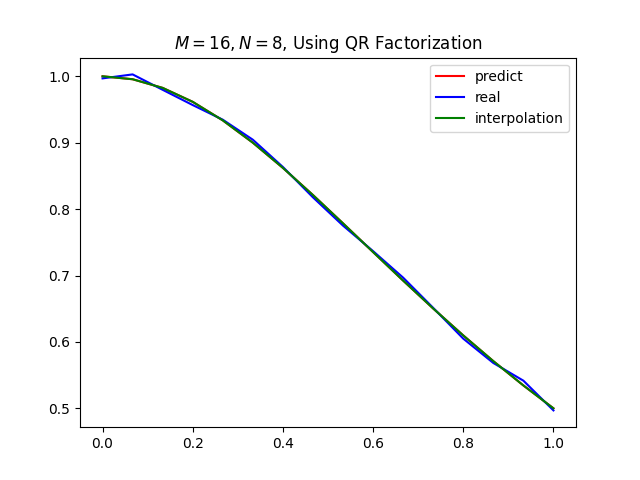
\includegraphics[width=1\textwidth]{./QR/M=16N=8F.png}
    		\caption{$g_F(M=16,N=8)$}
    	\end{minipage}
    \end{figure}
	Although the interpolation fits the target function better, it is likely that overfitting will occur when N is big. However, if N is set improperly, for example, N is too small, like Figure 16, the result might not be good enough. So, choosing proper N is very important.
\end{enumerate}


\end{document}
